\documentclass{standalone}
\usepackage{tikz}
\usepackage{amsmath}

\begin{document}

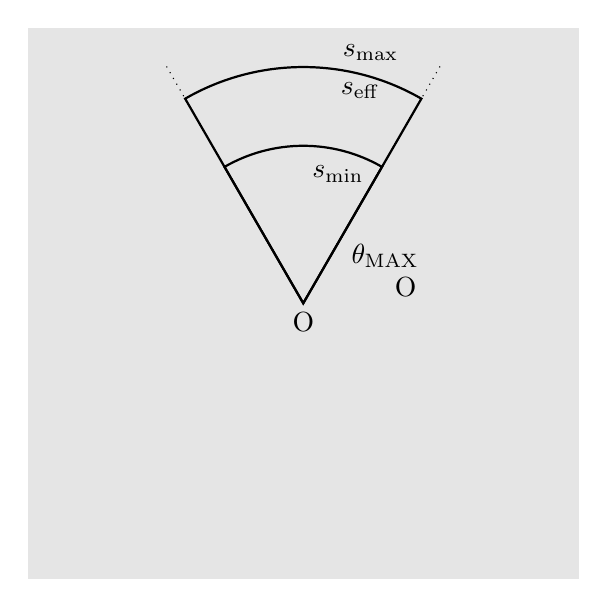
\begin{tikzpicture}
    % Background color
    \fill[gray!20] (-3.5,-3.5) rectangle (3.5,3.5);

    % Define radii
    \def\smin{2}
    \def\smax{3}
    \def\seff{2.5}
    \def\thetaMAX{60}

    % Draw arcs
    \draw[thick] (0,0) -- (\thetaMAX:\smin) arc (\thetaMAX:120:\smin) -- cycle;
    \draw[thick] (0,0) -- (\thetaMAX:\smax) arc (\thetaMAX:120:\smax) -- cycle;
    
    % Dashed line for effective distance
    \draw[dashed] (0,0) -- (\thetaMAX:\seff);
    
    % Draw dotted lines
    \draw[dotted] (0,0) -- (\thetaMAX:3.5);
    \draw[dotted] (0,0) -- (120:3.5);

    % Labels
    \node at (\thetaMAX/2:1.2) {$\theta_\mathrm{MAX}$};
    \node at (1.3,0.2) {O};
    \node at (75:\smin-0.3) {$s_\mathrm{min}$};
    \node at (75:\smax+0.3) {$s_\mathrm{max}$};
    \node at (75:\seff+0.3) {$s_\mathrm{eff}$};

    % Label for center
    \node[below] at (0,0) {O};
    
\end{tikzpicture}

\end{document}